\section{FEM}

\begin{figure}[!ht]
\centering
\subfloat[t][$\Delta_x = 0 mm$ e $\Delta_z = 0mm$]
{
	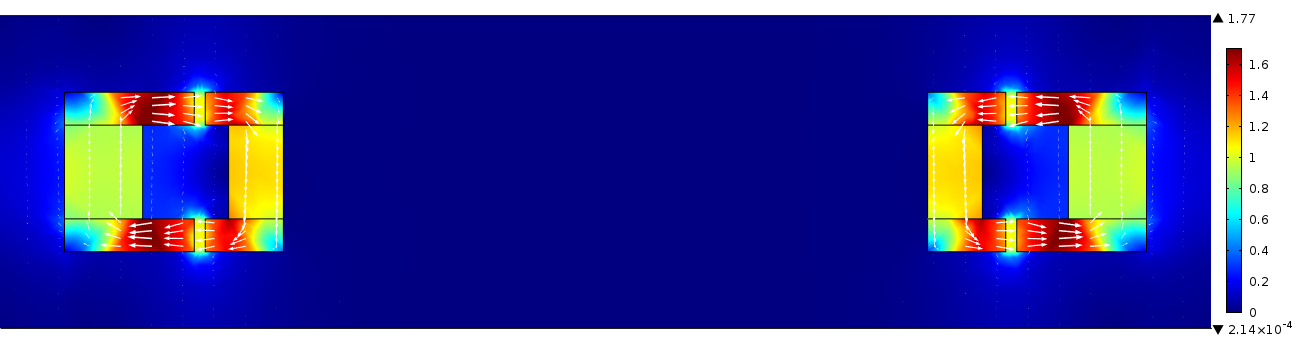
\includegraphics[width=1\linewidth]{Figs/Simulacoes/Passivo2/fem/dz00}
}	\\
\subfloat[t][$\Delta_x = 0.1 mm$ e $\Delta_z = 0mm$]
{
	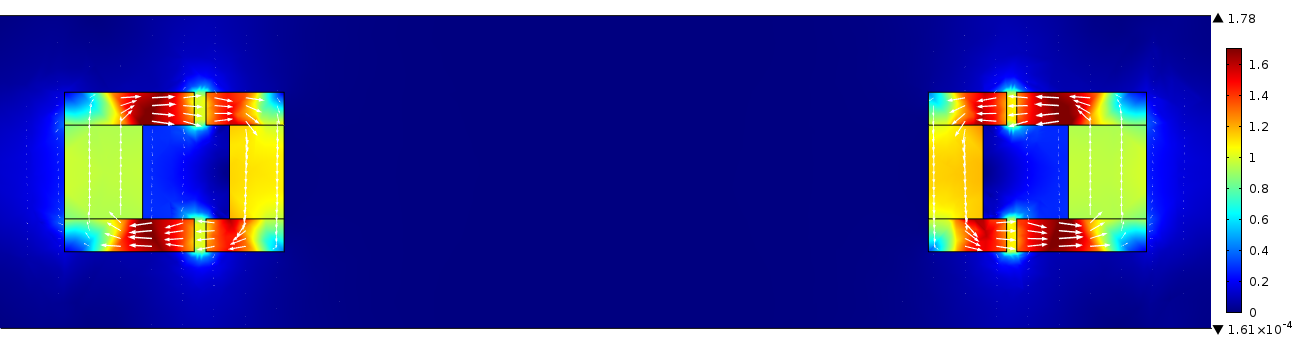
\includegraphics[width=1\linewidth]{Figs/Simulacoes/Passivo2/fem/dz01}
}	\\
\subfloat[t][$\Delta_x = 0.2 mm$ e $\Delta_z = 0mm$]
{
	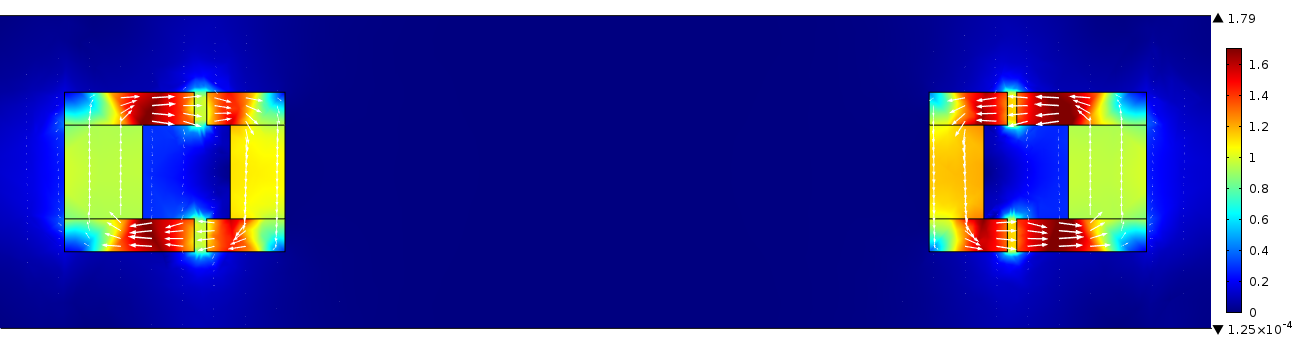
\includegraphics[width=1\linewidth]{Figs/Simulacoes/Passivo2/fem/dz02}
}	\\
\subfloat[t][$\Delta_x = 0.3 mm$ e $\Delta_z = 0mm$]
{
	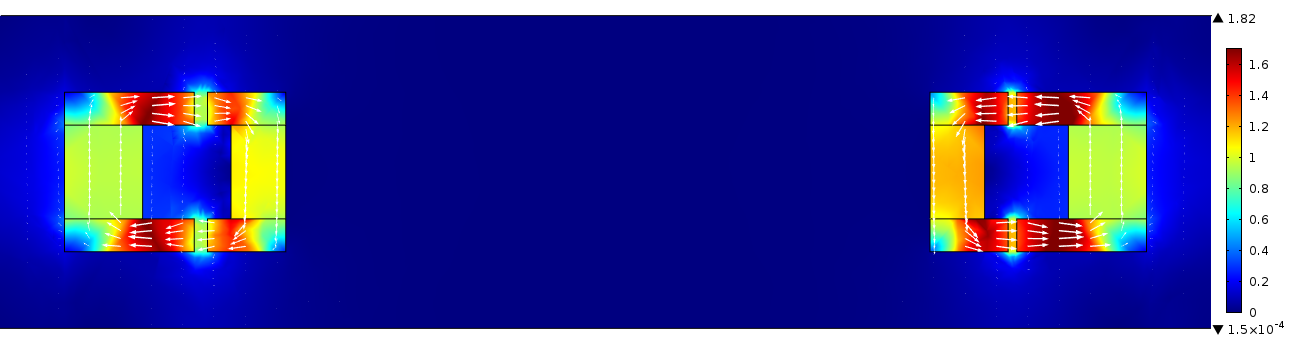
\includegraphics[width=1\linewidth]{Figs/Simulacoes/Passivo2/fem/dz03}
}	

\caption{Campo magnético via simulação em elementos finitos para deslocamentos radial}
\label{Fig:Modelagem:Curva:passivo:dx:linhas}
\end{figure}
